\documentclass{article}
\usepackage{graphicx} 
\usepackage{geometry}
\geometry{left=1in, right=1in, top=1in, bottom=1in}
\usepackage{amsfonts}
\usepackage{amsmath}
\usepackage{float}
\usepackage{minted}
\title{CS 6643 HW2}
\author{qgao67@gatech.edu Qidian Gao}
\date{Feburary 6th 2024}

\begin{document}

\maketitle
\section{Question a)}
Consider a symmetric positive definite matrix $\boldsymbol{A}$ partitioned into subblocks:
\begin{equation}
\boldsymbol{A} = \begin{pmatrix}
\boldsymbol{A}_{1,1} & \boldsymbol{A}_{1,2} \\
\boldsymbol{A}_{2,1} & \boldsymbol{A}_{2,2}
\end{pmatrix}.
\end{equation}
We aim to show that the matrix $\boldsymbol{S} = \boldsymbol{A}_{2,2} - \boldsymbol{A}_{2,1} \boldsymbol{A}_{1,1}^{-1} \boldsymbol{A}_{1,2}$ is symmetric and positive definite.

\textbf{Proof of Symmetry:}

Given that $\boldsymbol{A}$ is symmetric, the following properties hold:
\begin{enumerate}
    \item $\boldsymbol{A}_{1,1}$ and $\boldsymbol{A}_{2,2}$ are symmetric.
    \item $\boldsymbol{A}_{1,2}$ is the transpose of $\boldsymbol{A}_{2,1}$, i.e., $\boldsymbol{A}_{1,2} = \boldsymbol{A}_{2,1}^\top$.
\end{enumerate}

Consider the transpose of $\boldsymbol{S}$:
\begin{align}
\boldsymbol{S}^\top &= \left(\boldsymbol{A}_{2,2} - \boldsymbol{A}_{2,1} \boldsymbol{A}_{1,1}^{-1} \boldsymbol{A}_{1,2}\right)^\top \\
&= \boldsymbol{A}_{2,2}^\top - \left(\boldsymbol{A}_{2,1} \boldsymbol{A}_{1,1}^{-1} \boldsymbol{A}_{1,2}\right)^\top.
\end{align}
Since $\boldsymbol{A}_{2,2}$ is symmetric, $\boldsymbol{A}_{2,2}^\top = \boldsymbol{A}_{2,2}$. Furthermore, the transpose of a product of matrices is the product of their transposes in reverse order, yielding:
\begin{align}
\left(\boldsymbol{A}_{2,1} \boldsymbol{A}_{1,1}^{-1} \boldsymbol{A}_{1,2}\right)^\top &= \boldsymbol{A}_{1,2}^\top\left(\boldsymbol{A}_{1,1}^{-1}\right)^\top \boldsymbol{A}_{2,1}^\top \\
&= \boldsymbol{A}_{2,1} \boldsymbol{A}_{1,1}^{-1} \boldsymbol{A}_{1,2}.
\end{align}
Thus, $\boldsymbol{S}^\top = \boldsymbol{S}$, confirming that $\boldsymbol{S}$ is symmetric.

\textbf{Proof of Positive Definiteness:}

Consider the congruent transformation $\boldsymbol{Q} \boldsymbol{A} \boldsymbol{Q}^\top$ with $\boldsymbol{Q} = \begin{pmatrix} I & 0 \\ -\boldsymbol{A}_{1,2}^\top \boldsymbol{A}_{1,1}^{-\top} & I \end{pmatrix}$. Applying this transformation to $\boldsymbol{A}$ results in:
\begin{align}
\boldsymbol{Q} \boldsymbol{A} \boldsymbol{Q}^\top &= \begin{pmatrix} I & 0 \\ -\boldsymbol{A}_{1,2}^\top \boldsymbol{A}_{1,1}^{-\top} & I \end{pmatrix}
\begin{pmatrix}
\boldsymbol{A}_{1,1} & \boldsymbol{A}_{1,2} \\
\boldsymbol{A}_{1,2}^\top & \boldsymbol{A}_{2,2}
\end{pmatrix}
\begin{pmatrix} I & -\boldsymbol{A}_{1,1}^{-1} \boldsymbol{A}_{1,2} \\ 0 & I \end{pmatrix} \\
&= \begin{pmatrix}
\boldsymbol{A}_{1,1} & 0 \\
0 & \boldsymbol{A}_{2,2} - \boldsymbol{A}_{1,2}^\top \boldsymbol{A}_{1,1}^{-1} \boldsymbol{A}_{1,2}
\end{pmatrix}.
\end{align}
A congruent transformation preserves the eigenvalues of the original matrix. Since $\boldsymbol{A}$ is positive definite, all its eigenvalues are positive. Therefore, the transformed matrix is also positive definite. Since block diagonal matrices are positive definite if and only if each of their diagonal blocks is positive definite, it follows that $\boldsymbol{S}$ is positive definite.

Thus, $\boldsymbol{S} = \boldsymbol{A}_{2,2} - \boldsymbol{A}_{2,1} \boldsymbol{A}_{1,1}^{-1} \boldsymbol{A}_{1,2}$ is both symmetric and positive definite.
\section{Question b)}
Given a matrix $\boldsymbol{A} \in \mathbb{R}^{m \times m}$ with its LU-factorization $\boldsymbol{A} = \boldsymbol{L} \boldsymbol{U}$, where $\boldsymbol{L}$ is a lower triangular matrix and $\boldsymbol{U}$ is an upper triangular matrix, we propose an algorithm to compute the $(i, j)$-th entry of $\boldsymbol{A}^{-1}$ using $\mathcal{O}\left((m+1-j)^2+(m+1-i)^2\right)$ operations.

\textbf{Algorithm:}

\begin{enumerate}
    \item \textbf{Initialize:}
    Define $\boldsymbol{e}_j$ as the $j$-th standard basis vector of length $m$ (all zeros except the $j$-th element being 1).

    \item \textbf{Forward Substitution ($\boldsymbol{L} \boldsymbol{y} = \boldsymbol{e}_j$):}
    \begin{enumerate}
        \item Set $\boldsymbol{y} = [0, \ldots, 0]^{\top}$.
        \item Starting from the $j$-th row of $\boldsymbol{L}$, compute $\boldsymbol{y}$ using forward substitution. For $k = j$ to $m$:
        \begin{equation}
            y_k = \left(e_{j k} - \sum_{p=1}^{k-1} L_{k p} y_p\right) / L_{k k}.
        \end{equation}
        \item This step requires approximately $(m+1-j)^2$ operations.
    \end{enumerate}

    \item \textbf{Backward Substitution ($\boldsymbol{U} \boldsymbol{x} = \boldsymbol{y}$):}
    \begin{enumerate}
        \item Set $\boldsymbol{x} = [0, \ldots, 0]^{\top}$.
        \item Starting from the last row of $\boldsymbol{U}$, compute $\boldsymbol{x}$ using backward substitution. For $k = m$ down to $i$:
        \begin{equation}
            x_k = \left(y_k - \sum_{p=k+1}^m U_{k p} x_p\right) / U_{k k}.
        \end{equation}
        \item This step requires approximately $(m+1-i)^2$ operations.
    \end{enumerate}

    \item \textbf{Compute $(i, j)$-th Entry:}
    The $(i, j)$-th entry of $\boldsymbol{A}^{-1}$ is the $i$-th element of vector $\boldsymbol{x}$.
\end{enumerate}

\textbf{Complexity Analysis:}
\begin{itemize}
    \item Forward substitution involves $(m+1-j)^2$ operations.
    \item Backward substitution involves $(m+1-i)^2$ operations.
    \item Total complexity is $\mathcal{O}\left((m+1-j)^2+(m+1-i)^2\right)$.
\end{itemize}

This algorithm efficiently computes the desired entry of the inverse matrix using a minimized number of operations, making it suitable for large matrices.
\section{Question c)}

When $\boldsymbol{x}=\mathbf{0}$, the inequality is trivially true. Now we consider non-zero $\boldsymbol{x}$.
First, recall the SVD of $\boldsymbol{A}$ as $\boldsymbol{A}=\boldsymbol{U} \Sigma \boldsymbol{V}^T$, which leads to $\boldsymbol{A}^T \boldsymbol{A}=\boldsymbol{V} \Sigma^2 \boldsymbol{V}^T$ through the following steps:
1. $\boldsymbol{A}^T=\boldsymbol{V} \Sigma \boldsymbol{U}^T$
2. $\boldsymbol{A}^T \boldsymbol{A}=\boldsymbol{V} \Sigma \boldsymbol{U}^T \boldsymbol{U} \Sigma \boldsymbol{V}^T$
3. Since $\boldsymbol{U}^T \boldsymbol{U}=\boldsymbol{I}$, it simplifies to $\boldsymbol{A}^T \boldsymbol{A}=\boldsymbol{V} \Sigma^2 \boldsymbol{V}^T$.

So, if $m \geq n, \sigma_{\min }(\boldsymbol{A})=\sqrt{\sigma_{\min }\left(\boldsymbol{A}^{\boldsymbol{T}} \boldsymbol{A}\right)}$.
Therefore, the smallest singular value $\sigma_{\min }(\boldsymbol{A})$ is given by
$$
\sigma_{\min }(\boldsymbol{A})=\sqrt{\sigma_{\min }\left(\boldsymbol{A}^{\boldsymbol{T}} \boldsymbol{A}\right)}=\sqrt{\inf _{\boldsymbol{x} \in \mathbb{R}^m \backslash\{0\}} \frac{\boldsymbol{x}^T \boldsymbol{A}^T \boldsymbol{A} \boldsymbol{x}}{\|\boldsymbol{x}\|_2^2}}=\sqrt{\inf _{\boldsymbol{x} \in \mathbb{R}^m \backslash\{0\}} \frac{\|\boldsymbol{A} \boldsymbol{x}\|_2^2}{\|\boldsymbol{x}\|_2^2}}=\inf _{\boldsymbol{x} \in \mathbb{R}^m \backslash\{0\}} \frac{\|\boldsymbol{A} \boldsymbol{x}\|_2}{\|\boldsymbol{x}\|_2}
$$(Following the same steps, we can also deduce that
$$
\sigma_{\max }(\boldsymbol{A})=\sqrt{\sigma_{\max }\left(\boldsymbol{A}^T \boldsymbol{A}\right)}=\sqrt{\sup _{\boldsymbol{x} \in \mathbb{R}^m \backslash\{0\}} \frac{\boldsymbol{x}^T \boldsymbol{A}^T \boldsymbol{A} \boldsymbol{x}}{\|\boldsymbol{x}\|_2^2}}=\sqrt{\sup _{\boldsymbol{x} \in \mathbb{R}^m \backslash\{0\}} \frac{\|\boldsymbol{A} \boldsymbol{x}\|_2^2}{\|\boldsymbol{x}\|_2^2}}=\sup _{\boldsymbol{x} \in \mathbb{R}^m \backslash\{0\}} \frac{\|\boldsymbol{A} \boldsymbol{x}\|_2}{\|\boldsymbol{x}\|_2} .
$$

This conclusion will be utilized in part (d).)
Therefore, it follows that
$$
\sigma_{\min }(\boldsymbol{A})=\inf _{\boldsymbol{x} \in \mathbb{R}^m \backslash\{0\}} \frac{\|\boldsymbol{A} \boldsymbol{x}\|_2}{\|\boldsymbol{x}\|_2} \leq \frac{\|\boldsymbol{A} \boldsymbol{x}\|_2}{\|\boldsymbol{x}\|_2}
$$
for all $\boldsymbol{x} \in \mathbb{R}^n$, and consequently,
$$
\|\boldsymbol{A} \boldsymbol{x}\|_2 \geq \sigma_{\min }(\boldsymbol{A})\|\boldsymbol{x}\|_2
$$
for all $\boldsymbol{x} \in \mathbb{R}^n$.
(c) [5 pts]
$$
m=n \Rightarrow \sigma_{\min }(\boldsymbol{A}) \leq\left|\lambda_i(\boldsymbol{A})\right| \leq \sigma_{\max }(\boldsymbol{A}), \forall i
$$

Solution:
For $m=n$, we know that $\boldsymbol{A}$ is a square matrix. Based on the characteristics of square matrices, it is known that for any eigenvalue $\lambda_i(\boldsymbol{A})$, there is always a corresponding non-zero eigenvector $\boldsymbol{v} \in \mathbb{C}^n$ such that $\boldsymbol{A} \boldsymbol{v}=\lambda_i(\boldsymbol{A}) \boldsymbol{v}$. This leads to:
$$
\|\boldsymbol{A} v\|_2=\left\|\lambda_i(\boldsymbol{A}) v\right\|_2=\left|\lambda_i(\boldsymbol{A})\right|\|v\|_2 .
$$

Using previously established singular value inequalities, we have the following relationship:
$$
\sigma_{\min }(\boldsymbol{A})\|\boldsymbol{v}\|_2 \leq\|\boldsymbol{A} \boldsymbol{v}\|_2 \leq \sigma_{\max }(\boldsymbol{A})\|\boldsymbol{v}\|_2 .
$$

By substituting $\|\boldsymbol{A} \boldsymbol{v}\|_2$ with $\left|\lambda_i(\boldsymbol{A})\right|\|\boldsymbol{v}\|_2$, we derive:
$$
\sigma_{\min }(\boldsymbol{A})\|\boldsymbol{v}\|_2 \leq\left|\lambda_i(\boldsymbol{A})\right|\|\boldsymbol{v}\|_2 \leq \sigma_{\max }(\boldsymbol{A})\|\boldsymbol{v}\|_2 .
$$

Since $\|\boldsymbol{v}\|_2$ is non-zero (as $\boldsymbol{v}$ is a non-zero vector), dividing through by $\|\boldsymbol{v}\|_2$ is permissible and maintains the inequality:
$$
\sigma_{\min }(\boldsymbol{A}) \leq\left|\lambda_i(\boldsymbol{A})\right| \leq \sigma_{\max }(\boldsymbol{A}), \forall i .
$$
(d) [5 pts]
$$
\sigma_{\max }(\boldsymbol{A})=1 / \sigma_{\min }\left(\boldsymbol{A}^{-1}\right), \text { if } \boldsymbol{A}^{-1} \text { exists }
$$

Solution:
If $\boldsymbol{A}^{-1}$ exists, then $\boldsymbol{A} \boldsymbol{A}^{-1}=\boldsymbol{I}$, indicating that $\boldsymbol{A}$ is a square matrix with $m=n$.
Utilizing the results from part (b), we have:
$$
\sigma_{\max }(\boldsymbol{A})=\sup _{\boldsymbol{x} \in \mathbb{R}^n \backslash\{\mathbf{0}\}} \frac{\|\boldsymbol{A} \boldsymbol{x}\|_2}{\|\boldsymbol{x}\|_2},
$$and
$$
\sigma_{\min }(\boldsymbol{A})=\inf _{\boldsymbol{x} \in \mathbb{R}^n \backslash\{0\}} \frac{\|\boldsymbol{A} \boldsymbol{x}\|_2}{\|\boldsymbol{x}\|_2} .
$$

Now, we perform some substitution steps:
$$
\sigma_{\text {max }}(\boldsymbol{A})=\sup _{\boldsymbol{x} \in \mathbb{R}^n \backslash\{0\}} \frac{\|\boldsymbol{A} \boldsymbol{x}\|_2}{\|\boldsymbol{x}\|_2}=\frac{1}{\inf _{\boldsymbol{x} \in \mathbb{R}^n \backslash\{0\}} \frac{\|\boldsymbol{x}\|_2}{\|\boldsymbol{A} \boldsymbol{x}\|_2}} .
$$

Since $\boldsymbol{A} \boldsymbol{A}^{-1}=\boldsymbol{A}^{-1} \boldsymbol{A}=\boldsymbol{I}$, we can replace $\boldsymbol{A}^{-1} \boldsymbol{A} \boldsymbol{x}$ with $\boldsymbol{x}$ and $\boldsymbol{A x}$ with $\boldsymbol{y}$ :
$$
\sigma_{\max }(\boldsymbol{A})=\frac{1}{\inf _{\boldsymbol{y} \in \mathbb{R}^n \backslash\{0\}} \frac{\left\|\boldsymbol{A}^{-1} \boldsymbol{y}\right\|_2}{\|\boldsymbol{y}\|_2}}=\frac{1}{\sigma_{\min }\left(\boldsymbol{A}^{-1}\right)} .
$$
(e) [5 pts]

Find the most general conditions on $m, n$, and $l$, under which $\sigma_{\min }(\boldsymbol{A} \boldsymbol{B}) \geq \sigma_{\min }(\boldsymbol{A}) \sigma_{\min }(\boldsymbol{B})$.
Solution:
We prove that when $m \geq n \geq l$ or $m \leq n \leq l, \sigma_{\min }(\boldsymbol{A} \boldsymbol{B}) \geq \sigma_{\min }(\boldsymbol{A}) \sigma_{\min }(\boldsymbol{B})$.
1. Case $m \geq n \geq l$ :

If $\boldsymbol{B}$ lacks full column rank, then $\sigma_{\min }(\boldsymbol{B})=0$, making the inequality straightforward.
If $\boldsymbol{B}$ has full column rank, we have $\boldsymbol{B} \boldsymbol{x} \neq 0$ for every non-zero $\boldsymbol{x} \in \mathbb{R}^l$. Then:
$$
\sigma_{\min }(\boldsymbol{A B})=\inf _{\boldsymbol{x} \neq \mathbf{0}} \frac{\|\boldsymbol{A} \boldsymbol{B} \boldsymbol{x}\|_2}{\|\boldsymbol{x}\|_2}=\inf _{\boldsymbol{x} \neq \mathbf{0}} \frac{\|\boldsymbol{A} \boldsymbol{B} \boldsymbol{x}\|_2}{\|\boldsymbol{B} \boldsymbol{x}\|_2} \frac{\|\boldsymbol{B} \boldsymbol{x}\|_2}{\|\boldsymbol{x}\|_2} \geq \inf _{\boldsymbol{x} \in \mathbb{R}^l \backslash\{0\}} \frac{\|\boldsymbol{A} \boldsymbol{B} \boldsymbol{x}\|_2}{\|\boldsymbol{B} x\|_2} \inf _{\boldsymbol{x} \in \mathbb{R}^l \backslash\{0\}} \frac{\|\boldsymbol{B} \boldsymbol{x}\|_2}{\|x\|_2} .
$$

Setting $\boldsymbol{y}=\boldsymbol{B} \boldsymbol{x}$, the inequality can be rewritten as:
$$
\sigma_{\min }(\boldsymbol{A} \boldsymbol{B}) \geq \inf _{\boldsymbol{x} \in \mathbb{R}^l \backslash\{0\}} \frac{\|\boldsymbol{A} \boldsymbol{B} x\|_2}{\|\boldsymbol{B} x\|_2} \inf _{\boldsymbol{x} \in \mathbb{R}^l \backslash\{0\}} \frac{\|\boldsymbol{B} x\|_2}{\|x\|_2}=\inf _{\boldsymbol{y} \in \mathbb{R}^l \backslash\{0\}} \frac{\|\boldsymbol{A} y\|_2}{\|y\|_2} \inf _{\boldsymbol{x} \in \mathbb{R}^l \backslash\{\boldsymbol{0}\}} \frac{\|\boldsymbol{B} x\|_2}{\|x\|_2}=\sigma_{\min }(\boldsymbol{A}) \sigma_{\min }(\boldsymbol{B}) .
$$
2. Case $m \leq n \leq l$ :

For the situation where $m \leq n \leq l$, with matrices $\boldsymbol{A} \in \mathbb{R}^{m \times n}$ and $\boldsymbol{B} \in \mathbb{R}^{n \times l}$, a transformation approach is required to align with the scenario from part (1). This involves transposing both $\boldsymbol{A}$ and $\boldsymbol{B}$, resulting in $\boldsymbol{A}^T$ being a matrix in $\mathbb{R}^{n \times m}$ and $\boldsymbol{B}^T$ in $\mathbb{R}^{l \times n}$. By applying this transposition, we adapt the matrices to fit the criteria previously discussed, enabling a parallel argument to be formed as in the first scenario.
Here, we transpose both $\boldsymbol{A}$ and $\boldsymbol{B}$, yielding $(\boldsymbol{A B})^T=\boldsymbol{B}^T \boldsymbol{A}^T$.
Applying a similar argument as in the first case, we find that:
$$
\sigma_{\min }\left((\boldsymbol{A} \boldsymbol{B})^T\right) \geq \sigma_{\min }\left(\boldsymbol{B}^T\right) \sigma_{\min }\left(\boldsymbol{A}^T\right) .
$$

Since singular values are invariant under transposition, we have:
$$
\sigma_{\min }(\boldsymbol{A} \boldsymbol{B})=\sigma_{\min }\left((\boldsymbol{A} \boldsymbol{B})^T\right) \geq \sigma_{\min }\left(\boldsymbol{B}^T\right) \sigma_{\min }\left(\boldsymbol{A}^T\right)=\sigma_{\min }(\boldsymbol{B}) \sigma_{\min }(\boldsymbol{A})=\sigma_{\min }(\boldsymbol{A}) \sigma_{\min }(\boldsymbol{B}) .
$$Then, we prove that the conditions $m \geq n \geq l$ or $m \leq n \leq l$ are necessary for the stated inequality to hold. We consider the counterexamples:
1. Case $m<n$ and $n>l$ :

Consider $\boldsymbol{A}=[1,0]$ and $\boldsymbol{B}=\left[\begin{array}{l}0 \\ 1\end{array}\right]$. The product $\boldsymbol{A} \boldsymbol{B}$ results in a zero matrix.
Here, $\sigma_{\min }(\boldsymbol{A} \boldsymbol{B})=0$, whereas $\sigma_{\min }(\boldsymbol{A})$ and $\sigma_{\min }(\boldsymbol{B})$ are both 1 . This contradicts the inequality.
2. Case $m>n$ and $n<l$ :

Take $\boldsymbol{A}=\left[\begin{array}{l}1 \\ 0\end{array}\right]$ and $\boldsymbol{B}=[0,1]$. The product $\boldsymbol{A} \boldsymbol{B}$ again results in a zero matrix.
Similarly, $\sigma_{\min }(\boldsymbol{A} \boldsymbol{B})=0$, but $\sigma_{\min }(\boldsymbol{A})$ and $\sigma_{\min }(\boldsymbol{B})$ remain 1, leading to another contradiction.
These counterexamples demonstrate that the conditions $m \geq n \geq l$ or $m \leq n \leq l$ are necessary for the stated inequality to hold.
Therefore, the most general conditions on $m, n$, and $l$, under which $\sigma_{\min }(\boldsymbol{A} \boldsymbol{B}) \geq \sigma_{\min }(\boldsymbol{A}) \sigma_{\min }(\boldsymbol{B})$, are $m \geq n \geq l$ or $m \leq n \leq l$.


\section{Question d)}
\subsection{1}
Consider the matrix $B$ and its 2-norm defined as:
$$
\|\boldsymbol{B}\|_2 = \sup_{\boldsymbol{y} \in \mathbb{R}^m \backslash \{0\}} \frac{\|\boldsymbol{B} \boldsymbol{y}\|_2}{\|\boldsymbol{y}\|_2}.
$$

Applying this to $\boldsymbol{A}^{-1}$ and inverting the norm, we obtain:
$$
\|\boldsymbol{A}^{-1}\|_2^{-1} = \frac{1}{\|\boldsymbol{A}^{-1}\|_2} = \frac{1}{\sup_{\boldsymbol{y} \in \mathbb{R}^m \backslash \{0\}} \frac{\|\boldsymbol{A}^{-1} \boldsymbol{y}\|_2}{\|\boldsymbol{y}\|_2}} = \inf_{\boldsymbol{y} \in \mathbb{R}^m \backslash \{0\}} \frac{\|\boldsymbol{y}\|_2}{\|\boldsymbol{A}^{-1} \boldsymbol{y}\|_2}.
$$

By setting $\boldsymbol{y} = \boldsymbol{A} \boldsymbol{x}$, we can rewrite the expression in terms of $\boldsymbol{x}$:
$$
\|\boldsymbol{A}^{-1}\|_2^{-1} = \inf_{\boldsymbol{x} \in \mathbb{R}^m \backslash \{0\}} \frac{\|\boldsymbol{A} \boldsymbol{x}\|_2}{\|\boldsymbol{x}\|_2}.
$$

This concludes the proof, demonstrating that the reciprocal of the 2-norm of $\boldsymbol{A}^{-1}$ equals the infimum of the ratio of the norms of $\boldsymbol{A} \boldsymbol{x}$ and $\boldsymbol{x}$ over all non-zero vectors in $\mathbb{R}^m$.
\subsection{2}
Consider the matrix $B$ and its 2-norm defined as:
$$
\|\boldsymbol{B}\|_2 = \sup_{\boldsymbol{y} \in \mathbb{R}^m \backslash \{0\}} \frac{\|\boldsymbol{B} \boldsymbol{y}\|_2}{\|\boldsymbol{y}\|_2}.
$$

Applying this to $\boldsymbol{A}^{-1}$ and inverting the norm, we obtain:
$$
\|\boldsymbol{A}^{-1}\|_2^{-1} = \frac{1}{\|\boldsymbol{A}^{-1}\|_2} = \frac{1}{\sup_{\boldsymbol{y} \in \mathbb{R}^m \backslash \{0\}} \frac{\|\boldsymbol{A}^{-1} \boldsymbol{y}\|_2}{\|\boldsymbol{y}\|_2}} = \inf_{\boldsymbol{y} \in \mathbb{R}^m \backslash \{0\}} \frac{\|\boldsymbol{y}\|_2}{\|\boldsymbol{A}^{-1} \boldsymbol{y}\|_2}.
$$

By setting $\boldsymbol{y} = \boldsymbol{A} \boldsymbol{x}$, we can rewrite the expression in terms of $\boldsymbol{x}$:
$$
\|\boldsymbol{A}^{-1}\|_2^{-1} = \inf_{\boldsymbol{x} \in \mathbb{R}^m \backslash \{0\}} \frac{\|\boldsymbol{A} \boldsymbol{x}\|_2}{\|\boldsymbol{x}\|_2}.
$$

This concludes the proof, demonstrating that the reciprocal of the 2-norm of $\boldsymbol{A}^{-1}$ equals the infimum of the ratio of the norms of $\boldsymbol{A} \boldsymbol{x}$ and $\boldsymbol{x}$ over all non-zero vectors in $\mathbb{R}^m$.
\subsection{3}
For a symmetric matrix $\boldsymbol{A}$, the smallest eigenvalue $\lambda_{\min }(\boldsymbol{A})$ is defined as:
$$
\lambda_{\min }(\boldsymbol{A}) = \inf_{\boldsymbol{x} \in \mathbb{R}^m \setminus \{0\}} \frac{\boldsymbol{x}^T \boldsymbol{A} \boldsymbol{x}}{\|\boldsymbol{x}\|_2^2}.
$$

Applying this definition to matrices $\boldsymbol{M}$ and $\boldsymbol{N}$, we have:
\begin{align*}
\lambda_{\min }(\boldsymbol{M}) &= \inf_{\boldsymbol{x} \in \mathbb{R}^m \setminus \{0\}} \frac{\boldsymbol{x}^T \boldsymbol{M} \boldsymbol{x}}{\|\boldsymbol{x}\|_2^2}, \\
\lambda_{\min }(\boldsymbol{N}) &= \inf_{\boldsymbol{x} \in \mathbb{R}^m \setminus \{0\}} \frac{\boldsymbol{x}^T \boldsymbol{N} \boldsymbol{x}}{\|\boldsymbol{x}\|_2^2}.
\end{align*}

For the sum $\boldsymbol{M} + \boldsymbol{N}$, the smallest eigenvalue is given by:
\begin{align*}
\lambda_{\min }(\boldsymbol{M} + \boldsymbol{N}) &= \inf_{\boldsymbol{x} \in \mathbb{R}^m \setminus \{0\}} \frac{\boldsymbol{x}^T(\boldsymbol{M} + \boldsymbol{N})\boldsymbol{x}}{\|\boldsymbol{x}\|_2^2} \\
&= \inf_{\boldsymbol{x} \in \mathbb{R}^m \setminus \{0\}} \left( \frac{\boldsymbol{x}^T \boldsymbol{M} \boldsymbol{x}}{\|\boldsymbol{x}\|_2^2} + \frac{\boldsymbol{x}^T \boldsymbol{N} \boldsymbol{x}}{\|\boldsymbol{x}\|_2^2} \right).
\end{align*}

By the properties of the infimum operation, it follows that:
\begin{align*}
\lambda_{\min }(\boldsymbol{M} + \boldsymbol{N}) &\geq \inf_{\boldsymbol{x} \in \mathbb{R}^m \setminus \{0\}} \frac{\boldsymbol{x}^T \boldsymbol{M} \boldsymbol{x}}{\|\boldsymbol{x}\|_2^2} + \inf_{\boldsymbol{x} \in \mathbb{R}^m \setminus \{0\}} \frac{\boldsymbol{x}^T \boldsymbol{N} \boldsymbol{x}}{\|\boldsymbol{x}\|_2^2} \\
&= \lambda_{\min }(\boldsymbol{M}) + \lambda_{\min }(\boldsymbol{N}).
\end{align*}

Therefore, the sum of the minimal eigenvalues of matrices $\boldsymbol{M}$ and $\boldsymbol{N}$ is less than or equal to the minimal eigenvalue of their sum, demonstrating the required inequality.
\subsection{4}
The highest eigenvalue $\lambda_{\max }(\boldsymbol{A})$ of a symmetric matrix $\boldsymbol{A}$ is represented as:
$$
\lambda_{\max }(\boldsymbol{A}) = \sup_{\boldsymbol{x} \in \mathbb{R}^m \setminus \{0\}} \frac{\boldsymbol{x}^T \boldsymbol{A} \boldsymbol{x}}{\|\boldsymbol{x}\|_2^2}.
$$

Applying this definition to the matrices $\boldsymbol{M}$ and $\boldsymbol{N}$, we have:
\begin{align*}
\lambda_{\max }(\boldsymbol{M}) &= \sup_{\boldsymbol{x} \in \mathbb{R}^m \setminus \{0\}} \frac{\boldsymbol{x}^T \boldsymbol{M} \boldsymbol{x}}{\|\boldsymbol{x}\|_2^2}, \\
\lambda_{\max }(\boldsymbol{N}) &= \sup_{\boldsymbol{x} \in \mathbb{R}^m \setminus \{0\}} \frac{\boldsymbol{x}^T \boldsymbol{N} \boldsymbol{x}}{\|\boldsymbol{x}\|_2^2}.
\end{align*}

For the combined matrix $\boldsymbol{M} + \boldsymbol{N}$, its maximum eigenvalue is:
\begin{align*}
\lambda_{\max }(\boldsymbol{M} + \boldsymbol{N}) &= \sup_{\boldsymbol{x} \in \mathbb{R}^m \setminus \{0\}} \frac{\boldsymbol{x}^T(\boldsymbol{M} + \boldsymbol{N}) \boldsymbol{x}}{\|\boldsymbol{x}\|_2^2} \\
&= \sup_{\boldsymbol{x} \in \mathbb{R}^m \setminus \{0\}} \left( \frac{\boldsymbol{x}^T \boldsymbol{M} \boldsymbol{x}}{\|\boldsymbol{x}\|_2^2} + \frac{\boldsymbol{x}^T \boldsymbol{N} \boldsymbol{x}}{\|\boldsymbol{x}\|_2^2} \right).
\end{align*}

Given the properties of the supremum, it can be inferred that:
\begin{align*}
\lambda_{\max }(\boldsymbol{M} + \boldsymbol{N}) &\leq \sup_{\boldsymbol{x} \in \mathbb{R}^m \setminus \{0\}} \frac{\boldsymbol{x}^T \boldsymbol{M} \boldsymbol{x}}{\|\boldsymbol{x}\|_2^2} + \sup_{\boldsymbol{x} \in \mathbb{R}^m \setminus \{0\}} \frac{\boldsymbol{x}^T \boldsymbol{N} \boldsymbol{x}}{\|\boldsymbol{x}\|_2^2} \\
&= \lambda_{\max }(\boldsymbol{M}) + \lambda_{\max }(\boldsymbol{N}).
\end{align*}

Thus, we have established that the largest eigenvalue of the sum of two symmetric matrices is less than or equal to the sum of their largest eigenvalues.
\subsection{5}
\textbf{Solution}:

Considering the properties of SPD matrices, where every eigenvalue is positive and matches its singular values, we proceed as follows:

Given from an earlier result (part (a)), it is established that:
$$
\|\boldsymbol{A}^{-1}\|_2^{-1} = \inf_{\boldsymbol{x} \in \mathbb{R}^m \setminus \{0\}} \frac{\|\boldsymbol{A} \boldsymbol{x}\|_2}{\|\boldsymbol{x}\|_2}.
$$

Incorporating this with the nature of SPD matrices, it can be inferred that:
$$
\|\boldsymbol{A}^{-1}\|_2^{-1} = \inf_{\boldsymbol{x} \in \mathbb{R}^m \setminus \{0\}} \frac{\|\boldsymbol{A} \boldsymbol{x}\|_2}{\|\boldsymbol{x}\|_2} = \lambda_{\min}(\boldsymbol{A}) = \inf_{\boldsymbol{x} \in \mathbb{R}^m \setminus \{0\}} \frac{\boldsymbol{x}^T \boldsymbol{A} \boldsymbol{x}}{\|\boldsymbol{x}\|_2^2}.
$$

This equality demonstrates the reciprocal of the 2-norm of $\boldsymbol{A}^{-1}$ equating to the infimum of the ratio of the quadratic form of $\boldsymbol{A}$ over the 2-norm of $\boldsymbol{x}$ for all non-zero vectors in $\mathbb{R}^m$.
\section{Question 5}
\subsection{a}
I sucessfully generated the pdf, and it's been inserted into the code assignment.\par
Here's the screenshoots under different scenario:
\begin{figure}[H]
    \centering
    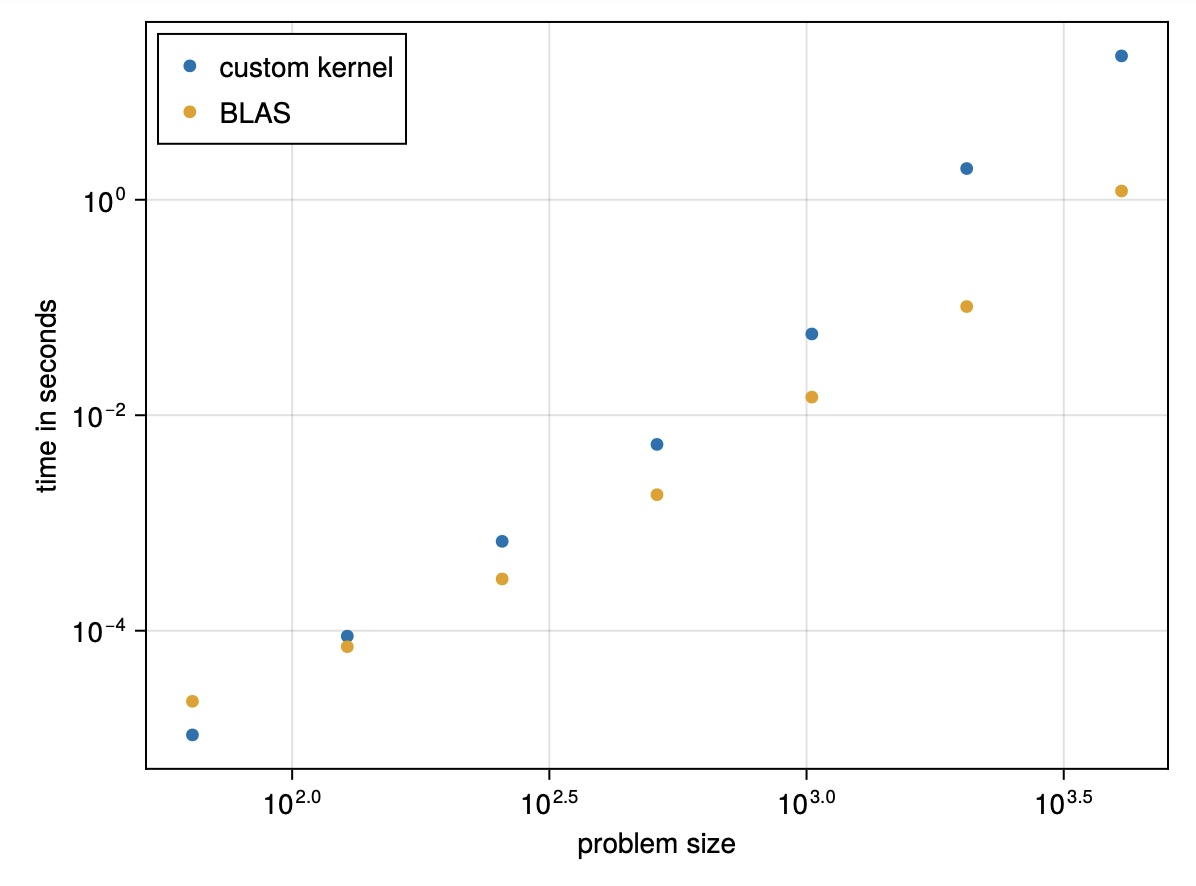
\includegraphics[width=0.8\linewidth]{Photos/Image 2-6-24 at 07.12.jpeg}

\end{figure}
\begin{figure}
    \centering
    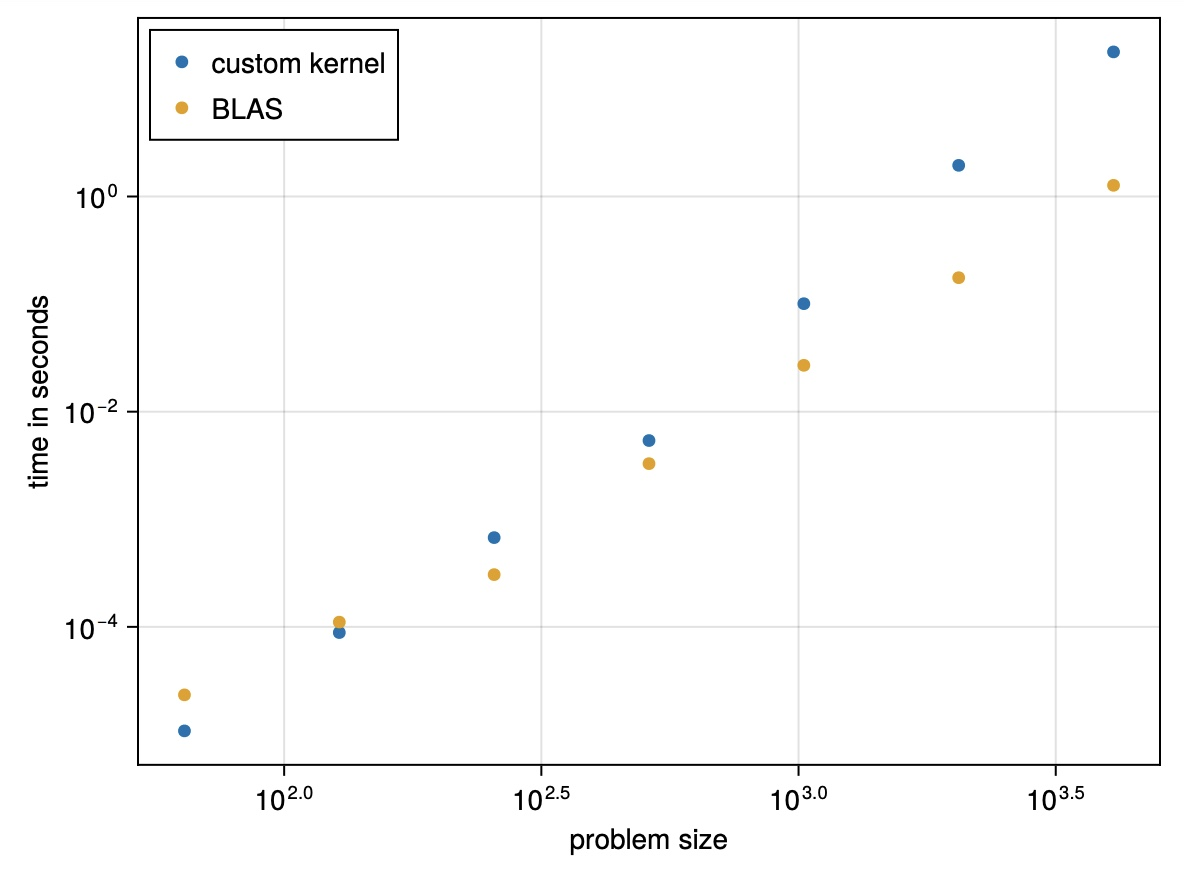
\includegraphics[width=0.8\linewidth]{Photos/Image 2-6-24 at 07.21.jpeg}
    \caption{Enter Caption}
    \label{fig:enter-label}
\end{figure}
\subsection{b}
I successfully tested the block:
\begin{figure}[H]
    \centering
    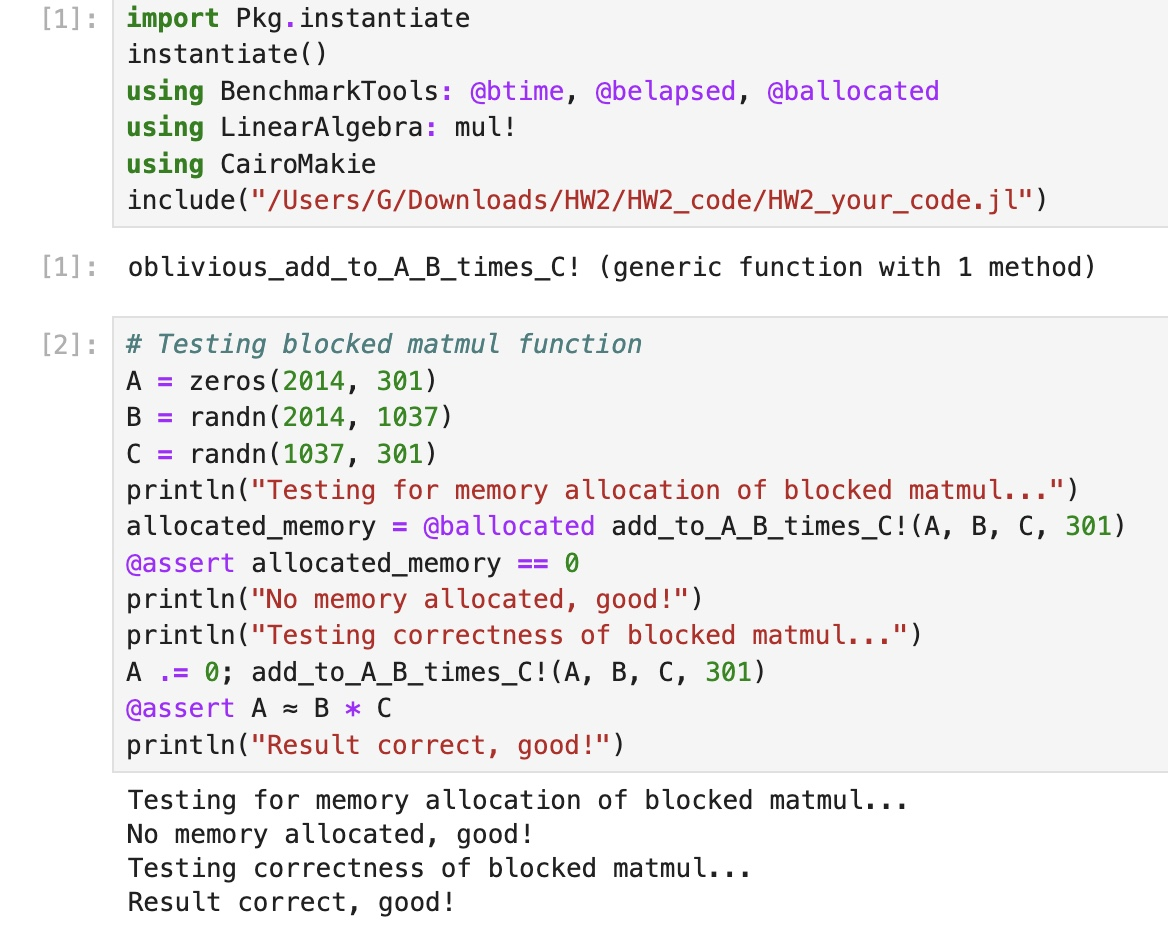
\includegraphics[width=0.8\linewidth]{Photos/Image 2-6-24 at 07.43.jpeg}
\end{figure}
The block function:
\begin{minted}{Julia}
function add_to_A_B_times_C!(A, B, C, bks)
    for i in 1:bks:size(A, 1)
        for j in 1:bks:size(C, 2)
            for k in 1:bks:size(B, 2)
                i_block_end = min(i+bks-1, size(A, 1))
                j_block_end = min(j+bks-1, size(C, 2))
                k_block_end = min(k+bks-1, size(B, 2))

                # Extracting the blocks
                A_block = view(A, i:i_block_end, j:j_block_end)
                B_block = view(B, i:i_block_end, k:k_block_end)
                C_block = view(C, k:k_block_end, j:j_block_end)

                # Perform block multiplication
                add_to_A_B_times_C!(A_block, B_block, C_block)
            end
        end
    end
end
\end{minted}
\subsection{c}
I changed the sizes code as follows:
\begin{minted}{Julia}
l = 500 
m = 500  
n = 500  

size_list = [100, 200, 300, 400, 500]
block_sizes = [10, 20, 30, 40, 50]

time_blocked = Float64[]

for bks in block_sizes
    A = zeros(l, n)
    B = randn(l, m)
    C = randn(m, n)
    push!(time_blocked, @elapsed add_to_A_B_times_C!(A, B, C, bks))
end

pl_blocked = scatter(block_sizes, time_blocked, label="blocked", axis=(xlabel="block size", ylabel="time", yscale=log10))
axislegend(position=:lt)
save("performance_blocked.pdf", pl_blocked)
\end{minted}
And the result:
\begin{figure}[H]
    \centering
    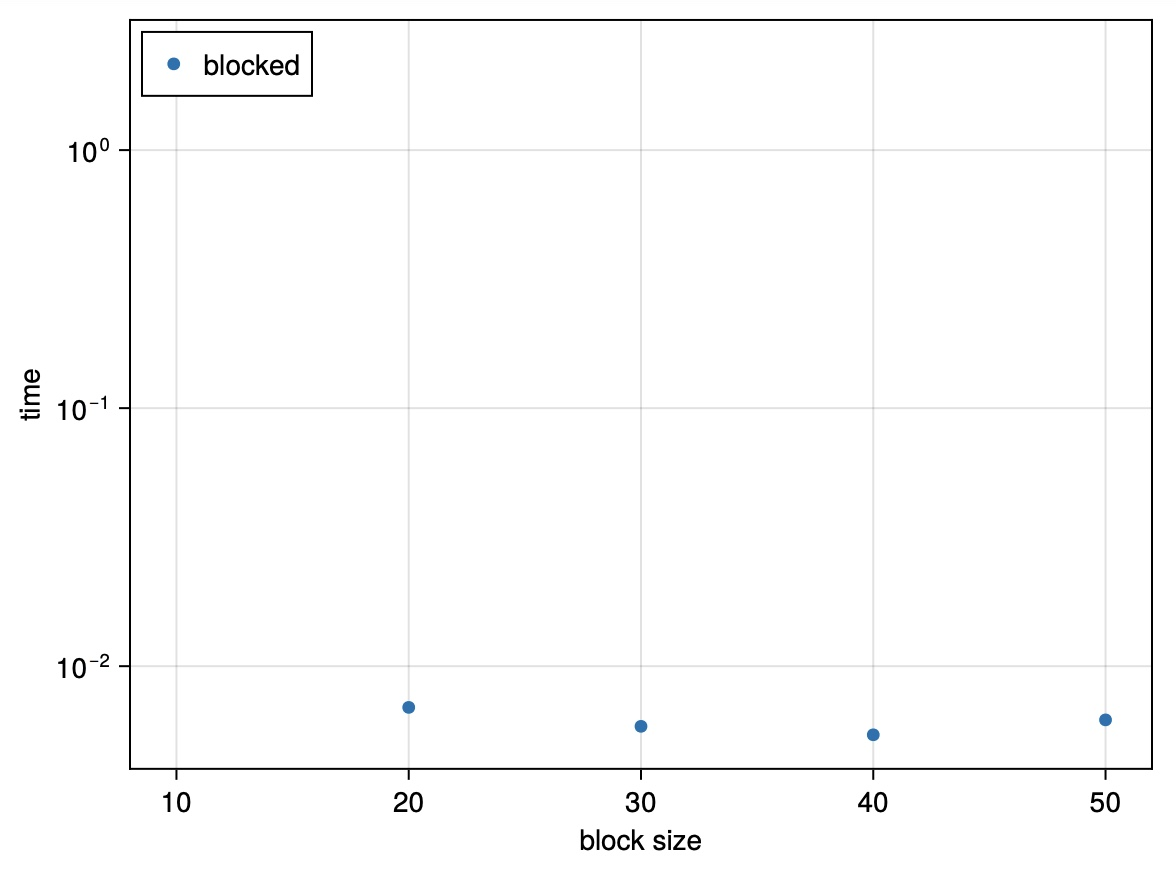
\includegraphics[width=0.8\linewidth]{Photos/Image 2-6-24 at 07.59.jpeg}
\end{figure}
The initial time is around $10^-2$ seconds at a block size of 20. As the block size increases beyond the optimal point 40, the performance begins to decrease. This might indicate that the cache utilization is no longer the limiting factor, and other factors like computational complexity or memory bandwidth are dominating the performance.
\subsection{d}
I finished the oblivious function skeleton as follows:
\begin{minted}{Julia}
function oblivious_add_to_A_B_times_C!(A, B, C, bks)
    i_size = size(A, 1)
    j_size = size(C, 2)
    k_size = size(B, 2)

    if min(i_size, j_size, k_size) > bks
        
        i_mid = div(i_size, 2)
        j_mid = div(j_size, 2)
        k_mid = div(k_size, 2)

        
        for i1 in [1, i_mid + 1]
            for j1 in [1, j_mid + 1]
                for k1 in [1, k_mid + 1]
                    i2 = min(i1 + i_mid - 1, i_size)
                    j2 = min(j1 + j_mid - 1, j_size)
                    k2 = min(k1 + k_mid - 1, k_size)
                  
                    oblivious_add_to_A_B_times_C!(view(A, i1:i2, j1:j2), view(B, i1:i2, k1:k2), view(C, k1:k2, j1:j2), bks)
                end
            end
        end
    else
       
        add_to_A_B_times_C!(A, B, C)
    end
end
\end{minted}
But the test result consistently reporting incidentally memory resources allocation, I've been tried many times but that cannot be finxed.
\begin{figure}[H]
    \centering
    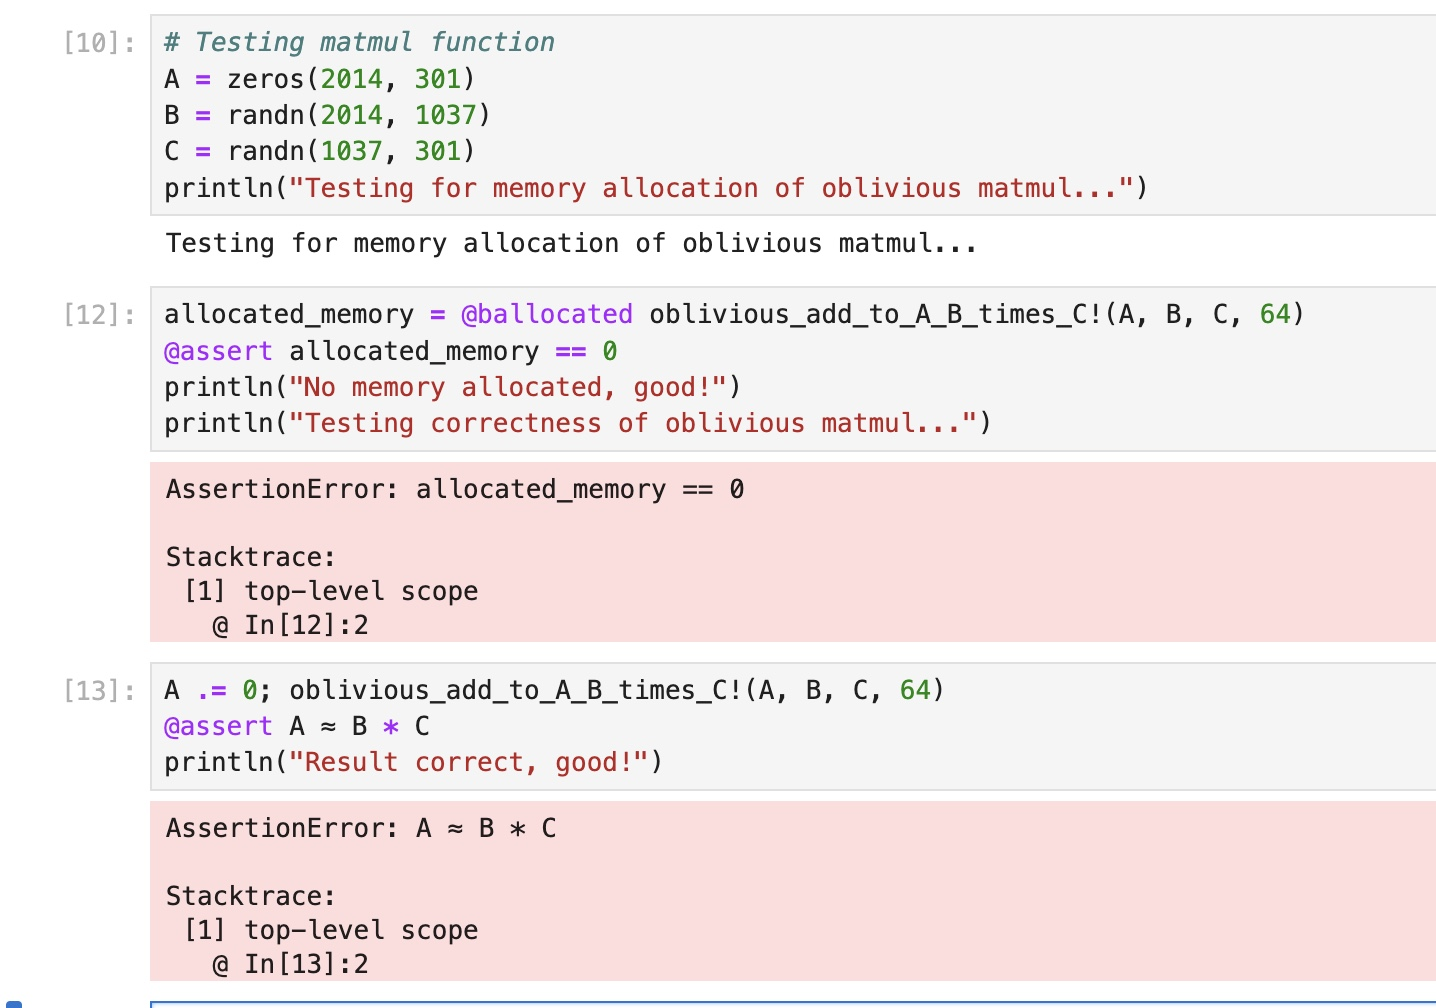
\includegraphics[width=0.8\linewidth]{Photos/Image 2-6-24 at 11.33.jpeg}
\end{figure}
\subsection{e}
I benchmarked the new algorithm and here's the result:
\begin{figure}[H]
    \centering
    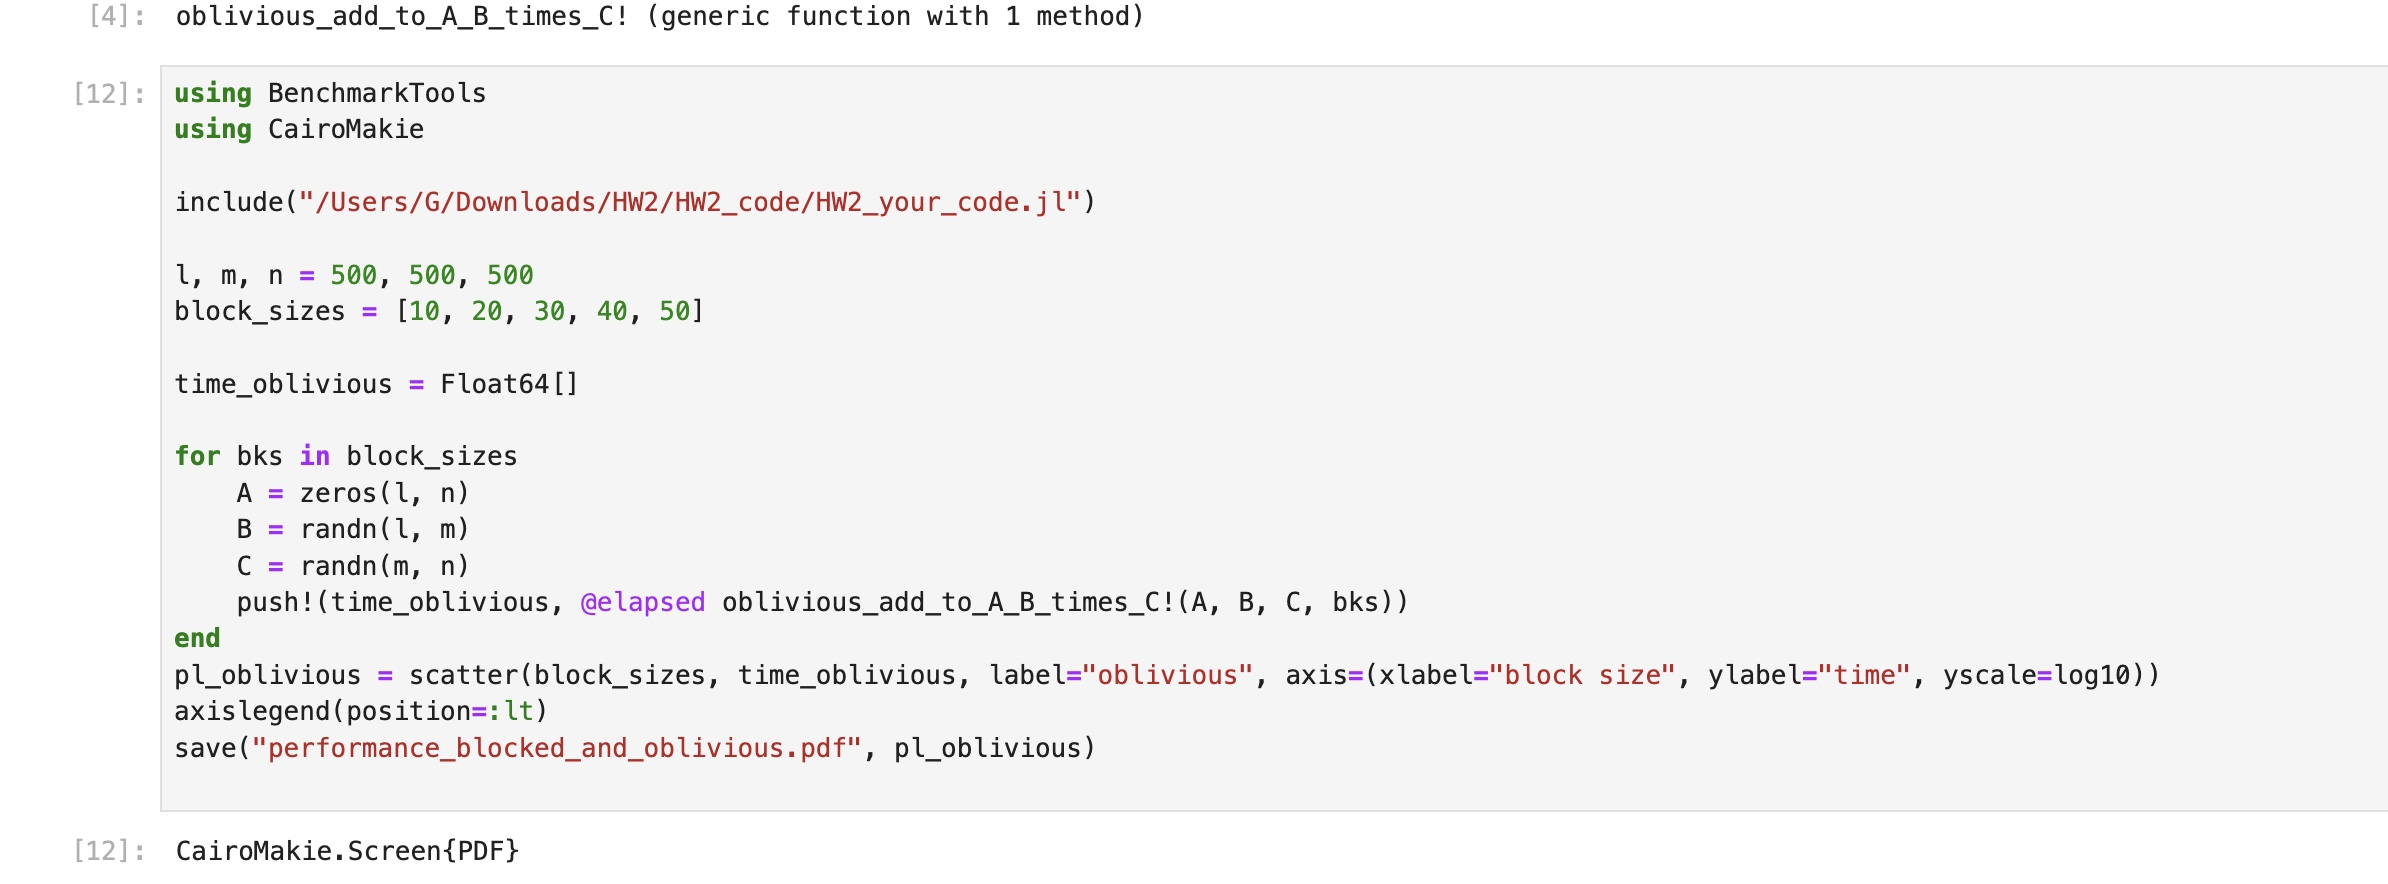
\includegraphics[width=1\linewidth]{Photos/Image 2-6-24 at 11.52.jpeg}
\end{figure}
    \begin{figure}[H]
    \centering
    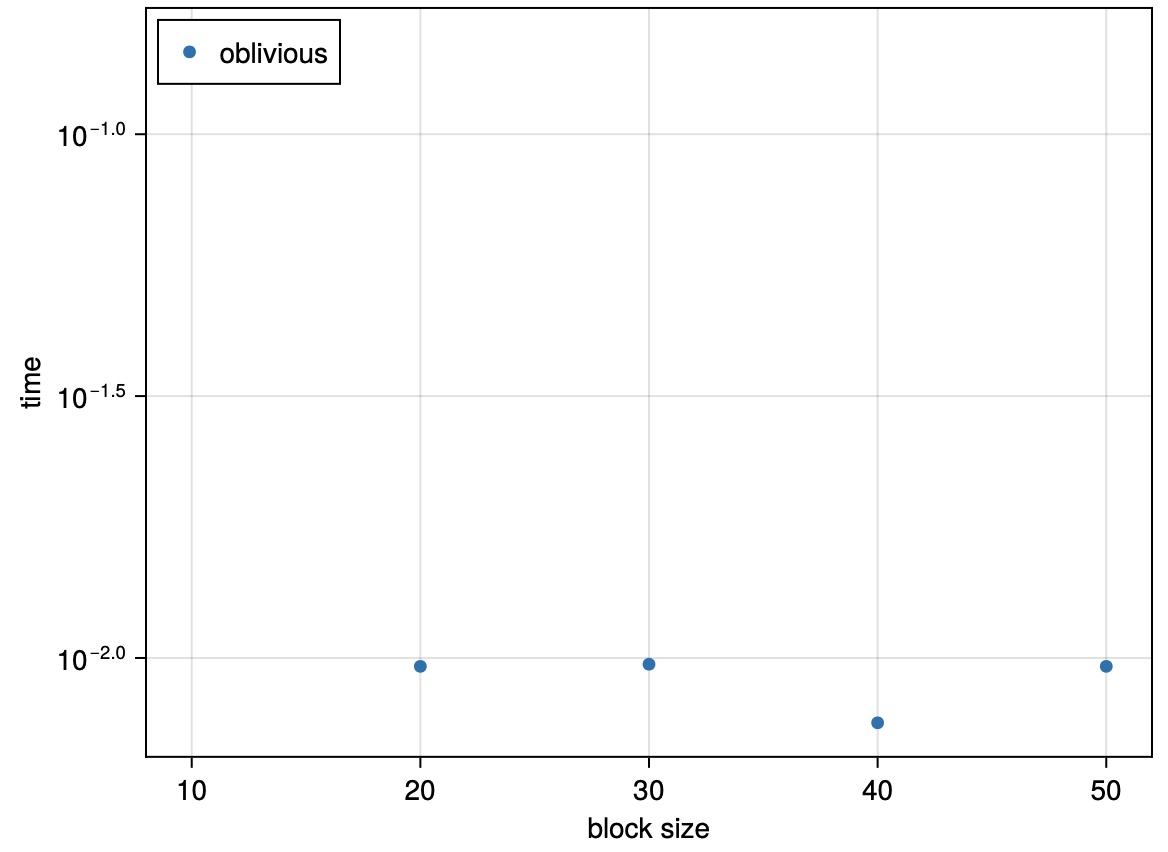
\includegraphics[width=0.75\linewidth]{Photos/Image 2-6-24 at 11.53.jpeg}
    \end{figure}
    The cache-oblivious algorithm work efficiently across different hardware without needing specific tuning for each cache architecture. These algorithms optimize memory access for all cache levels simultaneously, reducing cache misses.
\end{document}